\chapter{Gradient and categorical aspects of wordlikeness judgements} \label{gradience}

\citet{Halle1962} and \citet{Chomsky1965} observe that speakers internalize generalizations about possible and impossible words in their language. \citeauthor{Chomsky1965} illustrate this knowledge with two nonce words \emph{blick} [blɪk] and \emph{bnick} [bnɪk]. Whereas \emph{blick} is unattested, but in some sense a ``possible'' word of English, speakers immediately recognize \emph{bnick} to be ill-formed, an impossible word of the language.

A naïve account of this contrast is based on the assumption that segments or timing units must either be parsed into prosodic structures like the syllable, or be subject to phonological repair. Early precedents for this can be found in dissertations by \citet[10f.]{Hooper1973} and \citet[57f.]{Kahn1976}, and it is a fundamental component of many later frameworks \citep[e.g.,][]{Ito1989a,Noske1992,OT}. 

In English, [bl] is a permissible onset, but unlike some languages (e.g., Moroccan Arabic \emph{bni} `building', \emph{bnat} `daughters', \emph{bniqa} `closet'), [bn] is not. \citet[][19f.]{Wolf2009} suggest, for instance, that an underlying /bnɪk/ would be realized as [nɪk]; it is also possible to imagine resolution by prothesis---[əbnɪk]---or anapytxis---[bənɪk], and indeed \citet{Davidson2006b} finds that English speakers use all three of these repairs when asked to mimic foreign pronunciations of obstruent-nasal onsets like /bn/.

Many linguists who have concerned themselves with ``wordlikeness'' now regard the above as overly simplistic, for, as \citeauthor{Shademan2006} argues, such accounts draw a categorical boundary between the possible and impossible which fails to match the granularity at which speakers may report ``wordlikeness'' intuitions.

\begin{quote}
A defect of current grammatical acounts of phonotactics is that they render simple up-or-down decisions concerning well-formedness and cannot account for gradient judgements. But when judgements are elicited in a controlled fashion from speakers, they always emerge as gradient, including all intermediate values. \citep[][371]{Shademan2006} 
\end{quote}

This chapter focuses on the hypothesis, implicit in \citeauthor{Shademan2006}'s statement, that there is an inherent gradient or continuum between possible and impossible words, against an null hypothesis that the observed patterns of judgements are little more than an artifact of the wordlikeness task itself. \S\ref{2background} places this debate in a historical perspective, and argues that the naïve but widely accepted form of this hypothesis fails the test of falsifiability. In \S\ref{2evaluation}, a quantitative evaluation of a revised version of this hypothesis reveals a poor match between the gradience in speakers' judgements and contemporary computational models of wordlikeness. Taken together, the findings argue against the gradience hypothesis.

\section{Background} \label{2background}

\subsection{A brief history of the gradience hypothesis} \label{history}

\citeauthor{Chomsky1965} were not the first to consider the notion of possible and impossible words. Their primary contribution is that their mentalist perspective: they recognize that naïve speakers effortlessly acquire language-specific generalizations about possible and impossible words and can report them without any explicit training.

\subsubsection{The Copenhagen school}

Wordlikeness received some attention by structuralists of the Copenhagen school. In an early study, \citet{Fischer-Jorgensen1952} proposes that possible and impossible words represent endpoints on a continuum, and that no non-arbitrary line can be drawn between them. While it would anachronistic to assign this a mentalistic interpretation, this appears to be the earliest proposal that wordlikeness contrasts are in some sense gradient. 

However, not all early literature is concerned with gradience. \citet[][31]{Vogt1954}, for instance, recognizes that the taxonomic phoneme is insufficient to account for many wordlikeness contrasts. \citeauthor{Vogt1954} observes that allophony may account for the absence of certain phone sequences, but it does not provide a suitable explanation for the absence of initial [bn] in English, nor does it make correct predictions about the surface realization of an underlying initial /bn/. \citeauthor{Vogt1954} concludes that additional grammatical machinery will be needed to account for possible and impossible words. 

\subsubsection{Early generative grammar}

Gradient grammaticality is assumed in the earliest work on generative syntax, \emph{The logical structure of linguistic theory}, in which \citet[][132]{LSLT} writes that ``there is little doubt that speakers can fairly consistently order new utterances, never previously heard, with respect to their degree of `belongingness' to the language''. Later, \citet{ASPECTS} proposes that different syntactic violations give rise to different degrees of ungrammaticality. Unlike \citeauthor{Fischer-Jorgensen1952}, however, for \citeauthor{LSLT} this continuum does incorporate a hard-and-fast boundary between the grammatical and ungrammatical: there are no constrasts between grammatical utterances, merely between different degrees of ungrammaticality. For \citeauthor{LSLT}, all grammatical utterances are alike with respect to their grammaticality, but there are many degrees of ungrammaticality \citep[][61]{Schutze1996}.

\citet{Halle1962} and \citet{Stanley1967} concern themselves only with categorical wordlikeness contrasts, however. Both authors derive wordlikeness effects from morphophonemic redundancy rules acting on underlying representations. The discussion of \emph{bnick} by \citet[][101]{Chomsky1965} is a good example of this type of analysis. \citeauthor{Chomsky1965} observe that a consonant before a word-initial stop can only be a liquid in English. A corresponding redundancy rule which specifies a consonant in this position as [$+$\textsc{Liquid}] precludes the derivation of \emph{bnick}, since there is no way to realize the second consonant as a nasal.\footnote{This is not the only redundancy that could rule out \emph{bnick}. For instance, /s/ is the only word-initial obstruent that may precede a nasal consonant in English.}

\subsubsection{\emph{The sound pattern of English}} \label{2spe}

In \emph{The sound pattern of English} (Henceforth \emph{SPE}), \citet{SPE} argue that a complete solution to wordlikeness must countenance gradience. In addition to the contrast of \emph{blick} and \emph{bnick}, they introduce a third nonce word \emph{bnzk}, which they take to be even less well-formed than ``impossible'' \emph{bnick}. 

\begin{quote}
Hence, a real solution to the problem of ``admissibility'' will not simply define a tripartite categorization of occurring, accidental gap, and inadmissible, but will define the `degree of admissibility' of each potential lexical matrix in such a way as to\ldots{}make numerous other distinctions of this sort (\emph{SPE}:416--417)
\end{quote}

In some languages (e.g., Imdlawn Tashlhiyt Berber [tm.zħ] `she jested', [tzmt] `it (f.) is stifling'; \citealt{Dell1985}), \emph{bnzk} is syllabifiable, so its ill-formedness is once again a property of English, not a universal.

\citeauthor{SPE} propose to derive gradience from the complexity (using a simple feature-counting metric) of the redundancy rules needed to map a nonce word to an attested word, and they show that this derives the increasing cline of wordlikeness running from ``consonant soup'' \emph{bnzk} to ill-formed \emph{bnick}, possible \emph{blick}, and finally lexical \emph{brick}.

Despite the considerable attention given to the proposals of \emph{SPE} in the wake of that book's publication in 1968, the \emph{SPE} wordlikeness model has received almost no attention in the literature. At the risk of explaining what might be no more than an an accidental gap in the historical record, the novel aspects of the \emph{SPE} model---gradience derived from similarity to existing lexical entries---seem to have been overshadowed by compelling arguments against \citeauthor{SPE}'s assumption \citep[see also][]{Halle1962,Stanley1967} that wordlikeness contrasts derive from properties of underlying forms. \citet{Shibatani1973} observes that there are some generalizations about surface forms which give rise to wordlikeness contrasts, but cannot be stated as constraints on underlying forms. An example from German is shown in (\ref{fd}) below.

\begin{example}[German final devoicing] \label{fd}
\begin{tabular}{l l l l}
   & nom.sg. & nom.pl.    \\
a. & [piːp]    & [piːpə]  & `cheep(s)'      \\
   & [diːp]    & [diːbə]  & `thief/thieves' \\
b. & [ɡʀaːt]   & [ɡʀaːtə] & `ridge(s)'      \\
   & [ɡʀaːt]   & [ɡʀaːdə] & `degree(s)'     \\
\end{tabular}
\end{example}

\noindent The plural appears to preserve a contrast in final obstruent voicing which is absent in the singular:\footnote{While there is a contentious debate as to whether devoicing in German is completely neutralizing \citep[e.g.,][]{Fourakis1984}) or not \citep[e.g.,][]{Port1985}, it is irrelevant to the discussion at hand.} word-final voiced stops are never found in German, and \citet[95]{Shibatani1973} reports that ``it is easy to show that a native speaker of German rejects those forms \emph{on the ground that they end in voiced obstruents}'' (emphasis in original). However, given that root-final voicing is not predictable (e.g., /ɡʀaːt \alt{} ɡʀaːd/), the process of \textsc{Final Devoicing} cannot be any kind of lexical redundancy and is mysterious under the \emph{SPE} account. The alternative proposed by \citeauthor{Shibatani1973} and by \citet{Clayton1976}, is that to say that nonce words like [ɡʀaːd] are ill-formed not beacuse of any underlying property, but because they fail to undergo an otherwise-exceptionless phonological process, \textsc{Final Devoicing}, or equivalently, the surface-true generalization it derives.

\citet{Sommerstein1974} further notes that the computation of hypothetical underlying forms from nonce surface forms which is implied by the \emph{SPE} theory is non-trivial in the presence of phonological opacity \citep[see][528f.]{Anderson1988a}, and the rejection of the biuniqueness principle means that there is not always a unique solution, as is illustrated by the two underlying forms corresponding to [ɡʀaːt] in (\ref{fd}) above.

\subsubsection{Autosegmental phonology and beyond}

The arguments of \citeauthor{Shibatani1973} and others led theorists to focus their attention on properties of surface representations as determinants of wordlikeness. Though syllabification plays no role in \emph{SPE}, it is crucial to many earlier studies \citep[see][]{Goldsmith2011b}, and it received particular attention in the 1970s. \citet{Hooper1973} and \citet{Kahn1976} argue that the syllable is useful for defining wordlikeness generalizations.\footnote{\citet{Steriade1999} and \citet{Blevins2003}, however, argue that a number of phonotactic generalizations previously stated in syllabic terms can be reanalyzed without making reference to syllables.} \citeauthor{Hooper1973} argues, for instance, that [bn], impossible as an English onset, is unobjectionable as a syllable contact cluster in nonce words like \emph{stabnik} (or in names like \emph{Abner}), and that this demonstrates the superiority of syllable-based wordlikeness generalizations. This already signals further trouble for alternative accounts which focus on underlying forms. Syllabification may span morphs, is generally predictable, and is universally non-contrastive, and as a consequence, few posit in to be present in underlying representations \citep[though see, e.g.,][]{Vaux2003}. \citeauthor{Hooper1973} also points to loanword adaptations which produce native syllable structure \citep[e.g.,][]{Carlisle1991} as evidence that syllabification is part of the phonological computation. Further enrichments to the theory are provided by the autosegmental theory of the syllable \citep{McCarthy1979b}, which envisions the syllable as an articulated tree structure \citep[as envisioned by][]{Pike1947a}, and theories like prosodic licensing \citep{Ito1989a}, in which syllabification triggers phonological repairs.

While none of these authors discuss gradience, the syllable plays a role in the definition of a gradient measure, ``positional probability'', though to correlate closely with human judgements of wordlikeness. The positional probability of a nonce monosyllabic word is derived from the combined probabilities at which segments occur in onset, nucleus, and coda positions in the lexicon of a given language. 

Using the head-term preference paradigm, \citet{Jusczyk1993b} and \citet{Friederici1993} find that typically-developing children as young as 9 months of age distinguish between nonce words which are and are not phonotactically valid in their target language. \citet{Jusczyk1994} report that 9-month-old children acquiring English also show preferences for nonce words with high positional probability over those with low positional probability. Faciliatory effects of positional probability (i.e., shorter latencies) are reported for other nonce word tasks conducted with adults, including single-word shadowing \citep{Vitevitch1997,Vitevitch1998}, same/different judgements \citep{Vitevitch1999a,Luce2001,Lipinski2005,Vitevitch2005}, and lexical decision \citep{Pylkkanen2002a}.

Most relevant to the question at hand, \citet{Vitevitch1997} and \citet{Frisch2000} find that speakers' wordlikeness ratings of multisyllabic words are correlated wtih the positional probailities of the constituent syllables. Unfortunately, none of these researchers make any effort to eliminate the possibility that the low positional probability stimuli are ``impossible'' words of English. In fact, 
Chapter \ref{clusters} argues
%the author has argued elsewhere \citep{Gorman2012c}
that many of the stimuli used by \citet{Vitevitch1997} and \citet{Frisch2000} contain illicit word-medial consonant clusters. While \citeauthor{Vitevitch1997} neither control nor manipulate the well-formedness of medial clusters, in a post-hoc test they consider a probabilistic measure of cluster well-formedness, which reveals that cluster well-formedness is correlated with syllable-internal positional probabilities and the wordlikeness judgements. \citeauthor{Vitevitch1997} ultimately conclude that it cannot explain all the variation in wordlikeness. 

The aforementioned studies all conclude that the gradient measure of positional probability correlates with behavioral results. As the flaws of the \citet{Vitevitch1997} study demonstrate, the aforementioned studies do little to tease apart the gradient and categorical aspects of phonotactics. More generally, they do little to distinguish between positional probability and closely correlated measures like bigram probability (see \S\ref{bigram} below) or neighborhood density, since these studies carefully select stimuli which either have high or low values for all of positional probability, bigram probablility, and neighborhood density. This is particularly troublesome given that positional probability was created \emph{ex nihilo}; in contrast, the effects of neighborhood density in various psycholinguistic tasks are emergent properties of many models of speech production \citep[e.g.,][]{Luce1998,Luce2000} and perception \citep{Marslen-Wilson1984,Marslen-Wilson1987,McClelland1986,Norris1994,Norris2000}. 

\subsection{A naïve gradience hypothesis}

Recent critiques of this syllabification-based model focus on the existence of intermediate wordlikeness ratings \citep[see also][]{Coleman1997,Anttila2008}.

\begin{quote}
In the particular domain of phonotactics gradient intuitions are pervasive: they have been found in every experiment that allowed participants to rate forms on a scale.
\citep[][382]{Hayes2008a}

When native speakers are asked to judge made-up (nonce) words, their intuitions are rarely all-or-nothing. In the usual case, novel items fall along a gradient cline of acceptability. \citep[][9]{Albright2009a}
\end{quote}

As discussed in \S\ref{2spe} above, this is also the view of \citeauthor{SPE} in \emph{SPE}. The observation itself cannot be questioned, but \citeauthor{SPE}, \citeauthor{Hayes2008a}, and \citeauthor{Albright2009a} do not explicitly state why this data is relevant to the construction of models of wordlikeness. Presumably, these authors believe that these patterns of judgements demonstrate that wordlikeness, as an internal state, is gradient simply because subjects make use of intermediate degrees of wordlikeness in judgement tasks. This proposition, generalized below, is ``naïve'' not because it lacks sophistication, but because it is rooted in a belief in naïve realism, a philosophy which holds that perception provides a relatively direct picture of the nature of the world, an influential view in the cognitive sciences in general (see \citealt{Fodor1981a} for a critique).

\begin{unlabeledexample}
\textsc{Naïve Gradience Hypothesis}: If graded judgements of a concept or mental state use intermediate ratings, that concept or mental state is gradient
\end{unlabeledexample}

This proposition has the form of an indicative conditional. While the antecedent of this condition, the presence or absence of intermediate ratings in a graded judgement task, is readily observable, it has no bearing on the truth or falsity of the conditional proposition. However, whereas a false consequent (e.g., an all-or-nothing concept) would potentially falsify the proposition, the consequent, a mental state, cannot be directly observed. If this is the case, then both the proposition and the consequent (the proposition that wordlikeness is itself gradient) fail the test of falsification, placing it beyond the reach of scientific inquiry.

\citet{Armstrong1983} cut the Gordian knot by asserting the possibility of observing a false consequent; they find the existence of all-or-nothing concepts like ``odd number'' or (more controversially) ``female'' to be apparent.

\begin{quote}
Are there definitional concepts? Of course. For example, consider the concept \emph{odd number}. This seems to have a clear definition, a precise description\ldots{}No integer seems to sit on the fence, undecided as to whether it is quite even, or perhaps a bit odd. No odd number seems odder than any other odd number. \citep[274]{Armstrong1983}
\end{quote}

\citeauthor{Armstrong1983} note that if subjects produce intermediate ratings for these categories, then the naïve proposition is false, and this is what \citeauthor{Armstrong1983} find in their experiments. They ask subjects to rate, on a seven-point scale, the extent to which, e.g., certain odd counting numbers represent the concept ``odd number'', and find that speakers do make use of intermediate values, as can be seen in Figure \ref{agg}. In summary, the proposition that intermediate ratings indicate mental gradience is either untestable, or it is false, and is thus rejected.

\begin{figure} \centering
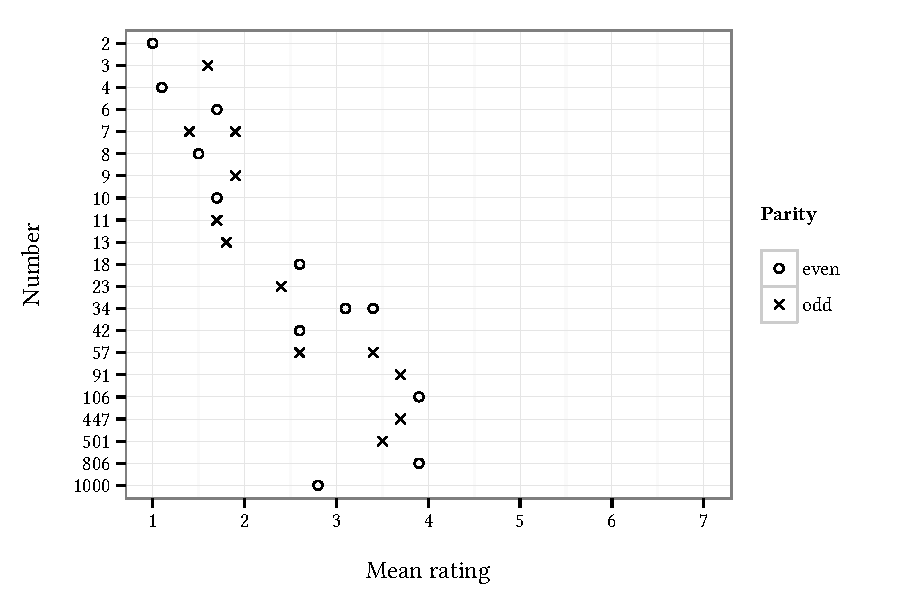
\includegraphics{agg.pdf}
\caption{Subjects asked to rate the degree to which certain even and odd numbers represent the categories ``even'' and ``odd'', respectively, freely use intermediate ratings.}
\label{agg} 
\end{figure}

\subsection{A falsifiable gradience hypothesis}

\citeauthor{Armstrong1983} do not view their results as evidence that subjects have an internal model of odd numbers which is at odds with the formal, all-or-nothing definition, and in fact, several additional experiments show that subjects deploy the extension of the formal definition in other tasks. Reviewing this study, \citet[215]{Schutze2011} writes that the experiments show that judgements are ``sensitive to factors other than our underlying competence''. In the case of wordlikeness, a case can be made that one such factor is similarity to existing words (e.g., \citealt[][151, fn. 27]{LSLT}, \citealt{Greenberg1964}, \citealt{Vitz1973}, \citealt{Ohala1986b}, \citealt{Sendlmeier1987}, \citealt{Bailey2001}, \citealt{Schutze2005}). However, the mere fact that subjects use intermediate ratings does not show that they do so with any systematicity, or that, e.g., the contrast between \emph{447} and \emph{7} with respect could be given any satisfying explanation. \citeauthor{Schutze2011} further suggests that gradience responses is a property of tasks, not concepts.

\begin{quote}
Putting it another way, when asked for gradient responses, participants will find some way to oblige the experimenter; if doing so is incompatible with the experimenter's actual question, they apparently infer that she must have really intended to ask something slightly different. \citep[][215]{Schutze2011}
\end{quote}

This introduces a troubling possibility, that subjects ``oblige'' experimenters by introducing random noise to their categorical judgements when presented with a Likert task. Were this the case, the observed intermediate judgements would scarcely be worthy of modeling. The alternative considered here is that there exists some model in which the gradience in ratings is systematic. 

\begin{unlabeledexample}
\textsc{Gradience Hypothesis}: If graded judgements of a concept or mental state use intermediate ratings, there is some model which can predict this behavior
\end{unlabeledexample}

\noindent There are now many computational models of wordlikeness which proport to do just this. An unfortunate defect of prior evaluations of these models, however, is that they adopt the naïve gradience hypothesis. \citet[382]{Hayes2008a} are just some of the authors who consider the ability to model gradient intuitions to be so important that they do not include any categorical models in their evaluation. As a result, the literature contains no serious attempt to evaluate the gradience hypothesis.

\section{Evaluation} \label{2evaluation}

The remainder of this chapter is devoted to testing the revised hypothesis. This is accomplished by an evaluation of computational models of wordlikeness in which categorical and gradient models are placed on an equal footing.

\subsection{Data sources}

The evaluation makes exclusive use of previously published English wordlikeness data. For inclusion in the evaluation, a study must conform to all three of the following conditions. First, the stimuli must consist only of monosyllabic words presented auditorily. Secondly, a significant portion of the stimuli must contain gross phonotactic violations (e.g., \emph{bnick}). Finally, the ratings, averaged across subjects, must be publicly available. The large-scale studies by \citet{Bailey2001} and \citet{Shademan2006,Shademan2007} are ineligible because the former lack stimuli with gross phonotactic violations and the latter data are not available to the public in any form. All data are reproduced in Appendix \ref{appendixA}.

\subsubsection{\citealt{Greenberg1964}}

\citet{Greenberg1964} investigated wordlikeness using the technique of free magnitude estimation, a mechanism which has become increasingly popular among syntacticians \citep[e.g.,][]{Bard1996}. At the beginning of the experiment, the subject heard a recording of the word \emph{stick}. In subsequent trials, the subjects heard a nonce word and were asked to report ``how far would you say that is from English?'', with \emph{stick} at ``1''; subjects are told that a word that is ``twice as far from English'' as \emph{stick} should be scored ``2''. The data used here are from \citeauthor{Greenberg1964}'s Experiment B, in which 17 undergraduates were presented 17 stimuli in all. In addition to \emph{stick}, the stimuli include three other English words; these four items were excluded from further analyses, leaving 13 stimuli. As is standard practice in psychophysics \citep[e.g.,][]{Butler1987}, these magnitude ratings were log-transformed before analysis.

\subsubsection{\citealt{Scholes1966}}

\citet{Scholes1966} conducted a number of English wordlikeness judgement with middle school children. The data used here come from his ``experiment 5'', in which 63 monosyllabic items were presented to 33 seventh-grade students. For each stimulus, the subjects produced forced choice ``yes''/``no'' answers to the question of whether the item ``is likely to be usable as a word of English''. \citet{Hayes2008a} and \citet{Albright2009a} analyze this data as gradient by performing an item averaging using the fraction of ``yes'' answers for each stimulus \citep[see also][]{Pierrehumbert1994,Coleman1997,Frisch2000}. For instance, 22 of the 33 students answered ``yes'' for \emph{shlerk} [ʃlɚk], so it is assigned a score of $0.666$.\footnote{This procedure conflates intraspeaker variation, which in some cases is considerable \citep{Shademan2007} with speaker-internal gradience, and its adoption here should not be construed as an endorsement. Rather, it is provided solely for comparison with prior studies using the \citeauthor{Scholes1966} data.} These stimuli are all ostensibly non-words, but include \emph{clung} [klʌŋ], the preterite and past participle of the verb \emph{cling}, and \emph{brung} [brʌŋ], a dialectical past participle for \emph{bring}. These two words were excluded and the remaining 61 stimuli were submitted to analysis. 

\subsubsection{\citealt{Albright2003b}}

\citet{Albright2003b} gathered wordlikeness judgements to serve as norms for a \emph{wug}-test. 87 items were presented to 20 undergraduate subjects, who rated each word on a seven-point Likert scale. The lowest point on the scale was labeled ``completely bizarre, impossible as an English word'', and that the highest point was labeled ``complete normal, would make a fine English word''.

\subsection{Model comparison}

The four models used here consist of a binary baseline and three computationally implemented gradient models. These three models are chosen because prior studies have shown they are correlated with wordlikeness judgements. Non-parametric rank correlation statistics are used evaluate the correlation between model predictions and wordlikeness ratings. Rank correlation are used rather than the parametric Pearson correlation statistic that is used by \citet{Hayes2008a}, for instance, because they make none of the potentially troublesome assumptions of the latter method \citep[see][23, fn. 12]{Albright2009a}.

The Spearman $\rho$ is most widely known rank correlation statistic, but it is difficult to give a natural interpretation to this quantity. On the other hand, the Kendall $\tau_b$ and Goodman-Kruskal $\gamma$ can be interpreted as fractions of the number of \emph{concordant} and \emph{discordant} pairs \citep{Noether1981}. Consider the case here, in which model scores are compared with wordlikeness ratings. If a model rates \emph{dresp} [dɹɛsp] more wordlike than *\emph{srest} [sɹɛst] and if speakers further rate \emph{dresp} more English-like than \emph{srest}, than \emph{dresp}/\emph{srest} are a concordant pair. If, however, a model and speakers disagree on the relative ranking of \emph{dresp} and \emph{srest}, the pair is discordant. The $\tau_b$ and $\gamma$ differ only in their treatment of ``ties'' (i.e., if e.g., *\emph{dresp} and *\emph{srest} are scored the same, or rated the same); $\tau_b$ includes a correction for ties, whereas $\gamma$ ignores tied pairs. Much like the familiar Pearson correlation, $\rho$, $\tau_b$ and $\gamma$ are all in the range [$-1$, $1$]. Correlations of the four models are given in Table \ref{cor}.

\begin{table} \centering
\begin{tabular}{l l l l l}
\toprule
Spearman $\rho$          & baseline         & maxent  & bigram           & density          \\
\midrule
\citealt{Greenberg1964}  & {0.845}          & {0.765} & {\textbf{0.863}} & {0.648}          \\
\citealt{Scholes1966}    & {0.791}          & {0.762} & {\textbf{0.827}} & {\textbf{0.827}} \\
\citealt{Albright2003b}  & {0.725}          & {0.429} & {0.708}          & {\textbf{0.742}} \\
\midrule
Kendall $\tau_b$         & baseline         & maxent  & bigram           & density          \\
\midrule
\citealt{Greenberg1964}  & {\textbf{0.716}} & {0.585} & {0.692}          & {0.462}          \\
\citealt{Scholes1966}    & {\textbf{0.664}} & {0.597} & {0.652}          & {0.565}          \\
\citealt{Albright2003b}  & {\textbf{0.599}} & {0.343} & {0.506}          & {0.556}          \\
\midrule
Goodman-Kruskal $\gamma$ & baseline         & maxent  & bigram           & density          \\
\midrule
\citealt{Greenberg1964}  & {\textbf{1.000}} & {0.684} & {0.692}          & {0.462}          \\
\citealt{Scholes1966}    & {\textbf{0.995}} & {0.634} & {0.667}          & {0.614}          \\
\citealt{Albright2003b}  & {\textbf{0.953}} & {0.656} & {0.509}          & {0.575}          \\
\bottomrule
\end{tabular}
\caption{Rank correlations between wordlikeness ratings and phonotactic models surprisingly reveal that the binary baseline meeds or exceeds the coverage of three state-of-the-art phonotactic models. All correlations are significant at $p = 0.05$.}
\label{cor}
\end{table}

\subsubsection{Binary baseline}

The binary baseline used here is a crude implementation of the null hypothesis that there are no gradient effects in wordlikeness judgements. To create such a baseline, it is necessary to distinguish between nonce words which contain a gross phonotactic violation and those which do not. As all stimuli here are monosyllables, this task can be further simplified by separately considering the two major subcomponents of the syllable, the onset and rime. Speakers are particularly adept as separating onsets from rimes \citep{Treiman1986,Treiman1995,Fowler1993}, and a large portion of phonotactic generalizations and violations can be localized to either onset or rime \citep[e.g.,][]{Fudge1969,Treiman1995,Kessler1997,Treiman2000}.

The baseline considers a nonce syllable to be well-formed if it consists of both an attested onset and an attested rime; the free combination of these two components is the only mechanism by which this model can generalize beyond attested words. It is surely the case that this is an ultimately insufficient model: \citet{Albright2009a} observes, for instance, that [ɛsp] is a well-formed rime, even though it is found in no word of English. This problem is more acute in languages with more permissive syllable structures than those of English, and thus a sparser lexicon with regard to phonotactic constraints. For instance, \citet{Fischer-Jorgensen1952} and \citet{Vogt1954} assert that there are many accidental gaps (i.e., possible but unattested structures) in the inventory of consonant clusters in Georgian, a language which admits as many as five adjacent consonants.\footnote{
%Chapter \ref{clusters} 
\citet{Gorman2012c}
reports a similar result for English syllable contact clusters.} Despite these defects, the baseline outperforms the gradient models in most contexts.

The rating densities from the three studies, linearly transformed to fit within the interval [0, 1] and split according to this binary baseline, are shown in Figure \ref{dsn}. In all three studies, it is possible to discern a relatively sharp separation between valid and invalid clusters, but also the presence of intermediate values.

\begin{figure} \centering
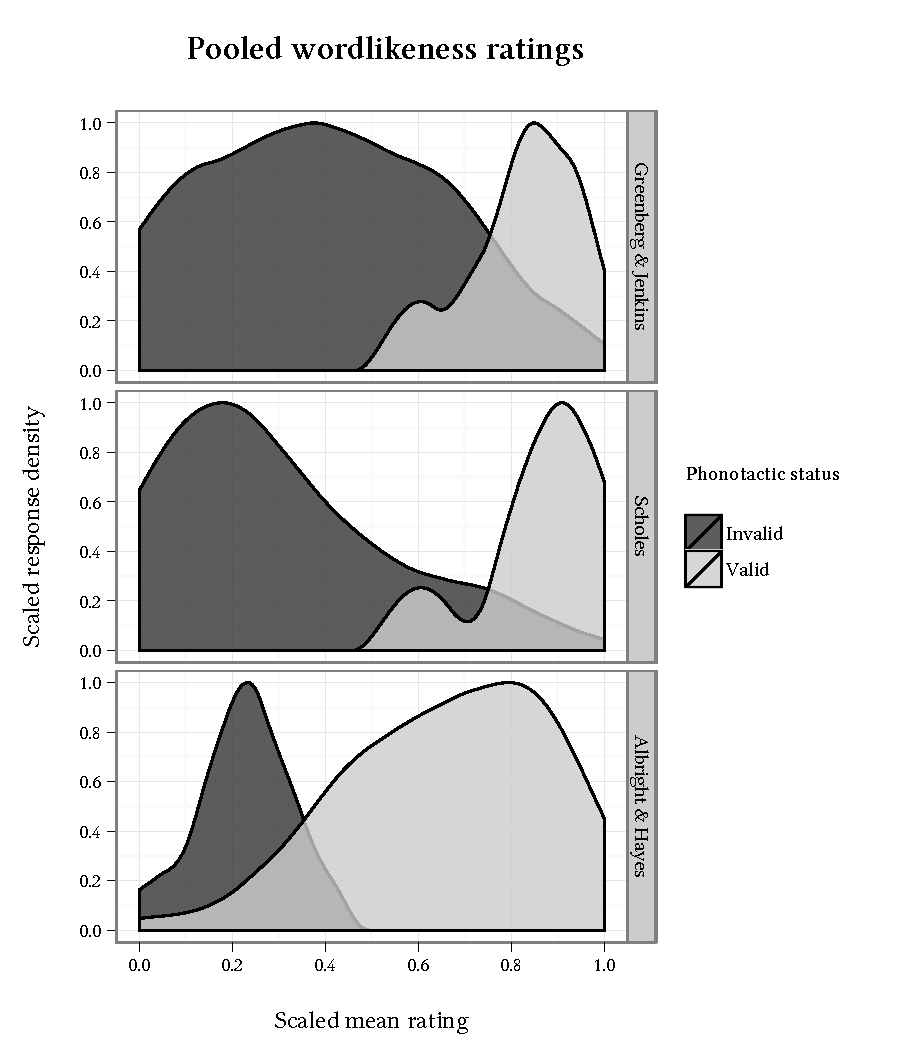
\includegraphics{density.pdf}
\caption{Average ratings of individual nonce words, linearly transformed to the interval [0, 1], tend to clump into two groups with little overlap; words which consist of  attested onsets and rimes receive ratings near ceiling, whereas ratings of phonotactically invalid words are spread across the lower half of the spectrum.}
\label{dsn}
\end{figure}

\subsubsection{Maximum entropy phonotactics}

\citeauthor{Hayes2008a} (\citeyear{Hayes2008a}; henceforth H\&W) develop a sophisticated model of phonotactic grammaticality which estimates a probability distribution over phoneme sequences by weighing constraints according to the principle of maximum entropy, following \citet{Goldwater2003} and \citet{Jager2007}. H\&W find that the predictions of their model are closely correlated with the \citet{Scholes1966} wordlikeness ratings. A direct replication of their predictions was attempted by using the software, model parameters, and training data as described in that study. Since the training of the maximum entropy model is inherently stochastic, producing slightly different outcomes on each run, the lowest scoring of ten runs is reported (H\&W:396), though in general there is not a great deal of variation between individual runs. One limitation of this model is that it is not feasible to score whole words, as the number of constraints which must be inspected grows exponentially as the size of possible constraints increases. Following H\&W and of \citet{Albright2009a}, who also applies the maximum entropy model to the \citet{Albright2003b} norms, the model is trained and scored only on stimulus onsets. However, as a consequence, the maximum entropy model performs particularly poorly on this data set, as many stimuli contain phonotactic violations in other positions.

\subsubsection{Segment bigram probability} \label{bigram}

The bigram probability of a sequence $ijk$ is the product of the probability of an sequence-initial $i$, the probability that $j$ follows $i$, and the probability that $k$ follows $j$, and the product of sequence-final \emph{k}.

\begin{unlabeledexample}
$\displaystyle \hat{p}(ijk) = p(i|\textrm{start}) \cdot p(j|i) \cdot p(k|j) \cdot p(\textrm{stop}|k)$
\end{unlabeledexample}

\noindent Bigram models are widely used in natural language processing, and \citet{Albright2009a} considers their relevance to modeling wordlikeness judgements. While the focus of \citeauthor{Albright2009a}'s study is on developing a model which uses bigrams over phonological features rather than segments themselves, \citeauthor{Albright2009a}'s evaluation, which includes both the \citeauthor{Scholes1966} and \citeauthor{Albright2003b} data sets, finds an advantage for segmental bigrams. 

\citeauthor{Albright2009a} estimates bigram probabilities using the method of maximum likelihood over types in the lexicon. The variant of segmental bigrams used here computes probabilities with a simple type of smoothing in which the count of all possible bigrams (including those never observed) are incremented by one. This technique is known as Laplace, or ``add one'' smoothing. This has the desirable effect that no nonce word is ever assigned a zero probability, and produces in a small increase in the correlation between the \citeauthor{Albright2003b} wordlikeness norms compared with the maximum likelihood estimate (Table \ref{albrightimproved}). For all three data sets, this model also consistenly outperforms positional probability models as defined by \citet{Vitevitch2004} and \citet{Vaden2009}. Given that these probabilities are highly correlatd with bigram probabilities \citep[][54]{Vitevitch1997}, they are not considered further. The bigram model consistently performs well in all the evaluations, and has the highest Spearman correlation with the \citeauthor{Greenberg1964} and \citeauthor{Scholes1966}, and is frequently second place model to the binary baseline elsewhere.

\begin{table} \centering
\begin{tabular}{l r r r}
\toprule
                         & maximum likelihood & Laplace smoothing \\
\midrule
Spearman $\rho$          & 0.660              & \textbf{0.708} \\
Kendall $\tau_b$         & 0.467              & \textbf{0.506} \\
Goodman-Kruskal $\gamma$ & 0.473              & \textbf{0.509} \\
\bottomrule
\end{tabular}
\caption{Laplace smoothing increases the correlation between the segmental bigram model proposed by \citet{Albright2009a}, which uses maximum likelihood estimation, and the \citet{Albright2003b} wordlikeness norms. All correlations are significant at $p = 0.05$.}
\label{albrightimproved}
\end{table}

\subsubsection{Neighborhood density} \label{density}

There are now many methods for computing similarity between nonce words and existing words, long thought to be reflected in wordlikeness judgements. 
For this study, a number of such methods were evaluated, including the Generalized Neighborhood Model \citep{Bailey2001}, PLD20 \citep{Suarez2011}, and a number of variations on neighborhood density \citep{Coltheart1977} provided by \citet{Vaden2009}. The best performance was obtained with the simplest version of neighborhood density, which is defined as the number of real monomorphemic words which can be changed into the target nonce word by a single insertion, deletion, or substitution of a phone.\footnote{\citet{Greenberg1964} use a variant in which only substitutions are counted.} For instance, the neighbors of \emph{blick} include \emph{blink} (insertion), \emph{lick} (deletion) and \emph{black} (substitution). While many studies \citep[e.g.,][]{Bailey2001} report robust lexical similarity effects, it may be that the relatively weak performance of neighborhood density is the result of the presence of gross phonotactic violations.

\subsection{Modeling residual gradience}

The primary result is that no gradient model reliably exceeds the accuracy of the binary baseline. Despite this, there are relatively strong correlations between the binary baseline and these gradient models (see Table \ref{bcor}). However, the fact that the gradient models are generally outperformed by the binary baseline suggest that they do not reliably predict intermediate ratings. To quantify this, the following method was used to estimate the residual contribution of the three gradient models once gross phonotactic violations are taken into account. Instead of calculating rank correlations directly on the model scores as in Table \ref{cor}, the model scores are mapped to ranks with the additional constraint that all ``valid'' stimuli be ranked above all ``invalid'' stimuli. The resulting ranks are used to compute new correlation statistics. Finally, the binary baseline correlation is subtracted from this number, so that the resulting value is the amount of improvement derived from augmenting the binary model with gradience. These difference numbers are shown in Table \ref{controlled}. In most cases, including the gradient models on top of the binary baseline produces a worse correlation than is obtained with the binary baseline alone.

For $\tau_b$ and $\gamma$, the interpretation of this result is clear. The gradient models assign rankings to the sets of phonotactically valid and invalid clusters, respectively. For instance, the bigram model favors \emph{troog} [tɹuːɡ] over \emph{swach} [swætʃ], though neither contains any gross phonotactic violation. Similarly, the bigram model favors \emph{chwoop} [tʃwuːp] over \emph{zhrick} [ʒɹɪk], even though neither word is a possible word of English. However, the majority of such predicted contrasts are not reflected in speakers' judgements; for instance, \emph{troog} is rated less English-like than \emph{swach} \citep{Greenberg1964}, contrary to the model predictions. This is stark evidence against the gradience hypothesis.

\begin{table} \centering
\begin{tabular}{l r r r}
\toprule
Kendall $\tau_b$          & maxent         & bigram         & density  \\
\midrule
\citealt{Greenberg1964}   & 0.670          & \textbf{0.680} & 0.501 \\
\citealt{Scholes1966}     & \textbf{0.685} & 0.632          & 0.639 \\
\citealt{Albright2003b}   & 0.542          & 0.603          & \textbf{0.623} \\
\bottomrule
\end{tabular}
\caption{The binary baseline is strongly correlated with the three gradient model scores; all correlations are significant at $p = 0.05$.}
\label{bcor}
\end{table}

\begin{table} \centering
\begin{tabular}{l r r r}
\toprule
$\Delta$ Spearman $\rho$          & maxent            & bigram            & density  \\
\midrule
\citealt{Greenberg1964}  & $-0.060$          &  \textbf{0.038} & $-0.017$ \\
\citealt{Scholes1966}    & $-0.029$          &  \textbf{0.047} & $-0.035$ \\
\citealt{Albright2003b}  & $-0.008$          & $-0.015$          & \textbf{0.018} \\
\midrule
$\Delta$ Kendall $\tau_b$         & maxent            & bigram            & density  \\
\midrule
\citealt{Greenberg1964}  & $-0.114$          & \textbf{$-$0.007} & $-0.084$ \\
\citealt{Scholes1966}    & $-0.067$          & \textbf{0.003}  & $-0.061$ \\
\citealt{Albright2003b}  & \textbf{$-$0.038} & $-0.092$          & $-0.049$ \\
\midrule
$\Delta$ Goodman-Kruskal $\gamma$ & maxent            & bigram            & density  \\
\midrule
\citealt{Greenberg1964}  & $-0.268$          & \textbf{$-$0.260} & $-0.337$ \\
\citealt{Scholes1966}    & $-0.361$          & \textbf{$-$0.313} & $-0.345$ \\
\citealt{Albright2003b}  & \textbf{$-$0.137} & $-0.443$          & $-0.386$ \\
\bottomrule
\end{tabular}
\caption{The change in rank correlation generated by augmenting the purely binary model with gradient predictions is small and in most cases it is negative.}
\label{controlled}
\end{table}

\section{Conclusions}

\subsection{The gradience hypothesis}

This chapter has evaluated the axiom of gradience as a falsifiable alternative hypothesis. The surprising result is that virtually all of the apparent coverage of state-of-the-art gradient phonotactic models is simply a reflection of their ability to distinguish between the possible and the totally impossible; beyond this, they are unreliable. A trivial baseline, endowed with few abilities to project beyond the observed data, generally outperforms the state of the art. It follows that the projections made by the state-of-the-art gradient models are not like those made by speakers. What remains to be seen is whether any model can be put forth which accurately predicts these intermediate ratings, and whether such a model deploys linguistic representations. 

These result provide support for recent findings that speakers asked to perform gradient syntactic judgements produce responses closely corresponding to a widely recognized categorical grammatical/ungrammatical distinction \citep{Sprouse2007}.

\subsection{Extensions to the binary baseline}

The strong performance of the binary baseline should not be taken as evidence either that wordlikenesss judgements are binary, or that the binary baseline is a plausible model. The most serious limitation of this evaluation is the primitive nature of the binary baseline. The inability to generalization within onsets and rimes is a serious flaw, as is the assumption of independence of onset and rime. A cognitively plausible version of this model must entertain phonotactic generalizations that are larger than these units.

A possible further extension to the binary baseline would be the introduction of additional levels of wellformedness. While the evaluation has shown that current gradient models do not reliably identify intermediate wellformedness, it does seem possible to identify at least three levels of grammaticality: for instance, one might share the intuition that \emph{zhlick} [ʒlɪk] is more similar to English than \emph{bnick}, though both have unattested onsets. 

There are precedents for labeling certain attested words as phonotactically ``peripheral'' (see, e.g., the appendices in \citealt{Myers1987} and \citealt{Borowsky1989}); such words are regarded as lexical exceptions to language-general principles of syllabification. If this extends to nonce words, then an intermediate level of grammaticality could be assigned to ``possible'' but formally marked words. Another likely source of additional levels of grammaticality is the cumulative effect of multiple phonotactic violations. While, as \citet{Coleman1997} note, classic model predict that a nonce word is as ill-formed as its worst deviation from syllable structure, it is possible to imagine that multiple phonotactic violations would result in greater degrees of ill-formedness. The bigram and maxent models make this prediction, as do many others \citep[e.g.,][]{Legendre1990,Levelt2000,Albright2008,Anttila2008,Pater2009b} but despite this, there is still little data demonstrating cumulative effects in wordlikeness tasks.

\subsection{Language acquisition}

The findings here also have interesting rammifications for language acquisition. \citet{Saffran1996} famously argues that infants use statistical dependencies between segments to extract words from continuous speech. Among those who ascribe to the Continuity Hypothesis \citep[e.g.,][]{Macnamara1982,Pinker1984,Crain1991,Carey1995,deVilliers2001,Legate2007}, which holds that children acquiring language deploy the same types of linguistic representations as adults, evidence for gradient phonotactic knowledge in infants is evidence for this knowledge in adults, and vis versa. The results here then stand to weaken the hypothesis of \citeauthor{Saffran1996}, as well as the hypothesis that infants acquire a system of phonotactics (gradient or otherwise) before learning of alternations and lexical entries that is a direct prediction of algorithms for learning Optimality Theory grammars \citep{Tesar2004,Hayes2004b}. 

%\footnote{The hypothesis that infants acquire a system of phonotactics (gradient or otherwise) before learning of alternations and lexical entries has some traction among formal linguists, for \citet{Hayes2004b} and \citet{Tesar2004} note that is a direct prediction of algorithms for learning Optimality Theory grammars. However, there is extensive evidence that infants who are younger than 9 months, the age at which \citet{Jusczyk1994} argue that the system probabilistic phonotactics comes online, have been demonstrated have already begun extracting words \citep[e.g.,][]{Darwin1877,Mandel1995,Jusczyk1995,Tincoff1999,Jusczyk1999b,Brent2001,Bortfeld2005,Seidl2006,Shukla2011,Bergelson2012} and alternations \citep{White2008} from multiword utterances they encounter.} Each of the tenets of this argument has been subject to serious critique, however.

First, it appears that children treat syllables holistically as early as 4 days after birth \citep{Bijeljac-Babic1993} and rapidly learn native-language syllable-based phonotactics \citep{Onishi2002,Chambers2003}, suggesting that any co-occurrence statistics should be delimited on units larger than the segments proposed by \citeauthor{Saffran1996}. Secondly, a good deal of the literature has focused on segmentation according to near exceptionless constraints that hold between adjacent syllables. For instance, infants as young as 4.5 months seem to be aware that English nasal codas agree in place with following obstruents \citep{Mattys2001b,Jusczyk2002,Davidson2004}. It might be the case that syllable co-occurrence statistics might be little more than a reflection of infants' learning of categorical ``lexical viability'' constraints \citep{Johnson2003} of the sort also seen in adult speech processing \citep[e.g.,][]{Norris1997}. Further, the effect of these statistical dependencies appear to be filtered by expectations about word stress \citep{Johnson2001,Mattys2001a,Shukla2007}, word length \citep{Lew-Williams2012}, and allophonic generalizations \citep{Hohne1994,Jusczyk1999c}. Finally, and perhaps most importantly, \citet{Gambell2005} find that a word segmentation strategy based only on statistical dependencies performs very poorly on realistic data. The emerging view of the role on statistics seems to be that infants attend to transitional probabilities or an analogue thereof only when they are faced with artificial stimuli with few of the properties of natural language \citep[e.g.,][]{Shukla2007,Lew-Williams2011}. The argument from Continuity is weak, in either direction.
